\documentclass[a4paper, 10pt, titlepage]{article}
\usepackage[utf8]{inputenc}
\usepackage[top=32mm, right=24mm, left=24mm]{geometry}
\usepackage{indentfirst}
\usepackage{graphicx}

\title{\textbf{ECSE-487 \\ COMPUTER ARCHITECTURE LABORATORY \\ Assignment \#1}}
\author{Andrei Purcarus \\ 260631911}
\date{January 30, 2017}

\begin{document}

\maketitle

\section{Introduction}

This report describes the design, simulation and synthesis of an image processing module that can parse PGM ASCII images byte by byte, store them in an internal memory block, perform pixel by pixel operations on them, and save the resulting images to files byte by byte in the same format. The processor is then applied to simulate an edge detector on sample images to demonstrate proof of concept.

\section{Design Description}

\subsection{SRAM}

First, a basic SRAM module was designed to store the pixels of the images being processed. Due to the size constraints of FPGA devices in terms of memory cells, a maximal image size of 255 by 255 8-bit pixels was decided upon for the simulation. In practical systems, the memory cells could be external DRAM cells, with SRAM caches for performance. This would allow for larger images to be stored.

A pin-out diagram of the component is shown in Figure \ref{fig:sram}. The component was made generic in terms of address width and data width in order to simplify reuse. The component is synchronized to the rising edge of the clock. To read data from the memory block, the address of the data is set, and the read\_en signal is asserted. On the next rising edge, the data will be available on the data\_out line. Similarly, to write data, the address to write to and the data\_in are set, and the write\_en signal is asserted. On the next rising edge, the data will be stored at the specified address. The processor system described in this report uses ADDR\_WIDTH = 16 and DATA\_WIDTH = 8 in order to satisfy the maximum image size described above.

\begin{figure}
    \centering
    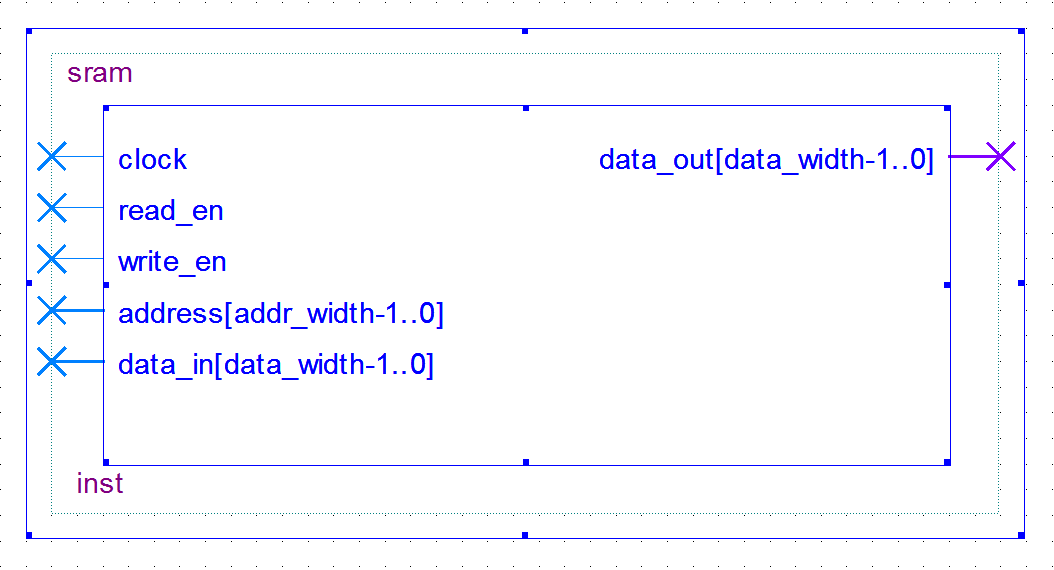
\includegraphics[width=0.5\linewidth]{sram_entity.PNG}
    \caption{An SRAM module designed to store images.}
    \label{fig:sram}
\end{figure}

\subsection{Image IO}

Next, the image IO modules were designed. In order to make these designs synthesizable, the actual file manipulation is left to the simulation test-benches. The load module assumes that a continuous byte input stream is available as input, and writes its data to an SRAM block as defined in the previous section. The save module assumes that its input is available in an SRAM block and that its output will be written to file when it asserts a signal.

A pin-out of the image load module is shown in Figure \ref{fig:image_load}. The design uses a datapath/controller system to parse a PGM image file. The data is fed continuously into the input on each rising clock edge, and the load\_en flag is asserted for as long as there is data available in the file. The module checks that the file satisfies the PGM image format as it loads data, and outputs an error code if it detects a violation. The possible error codes are described in Table \ref{tab:io_error}, and are defined in the image\_io\_error package. The pixel data is gradually output as the file is parsed, with the address and write\_en lines designed to store the data contiguously in an SRAM block. When the done flag is asserted, the img\_width, img\_height and maxval signals will contain the correct values assuming no errors, and the data will have been written to memory. The module then needs to be reset through the asynchronous reset flag to be able to parse another file. Internally, the module discards non-numeric data and comments and stores numeric data in a register, incrementing it as more digits are read before writing it to memory when a whitespace character is reached.

\begin{figure}
    \centering
    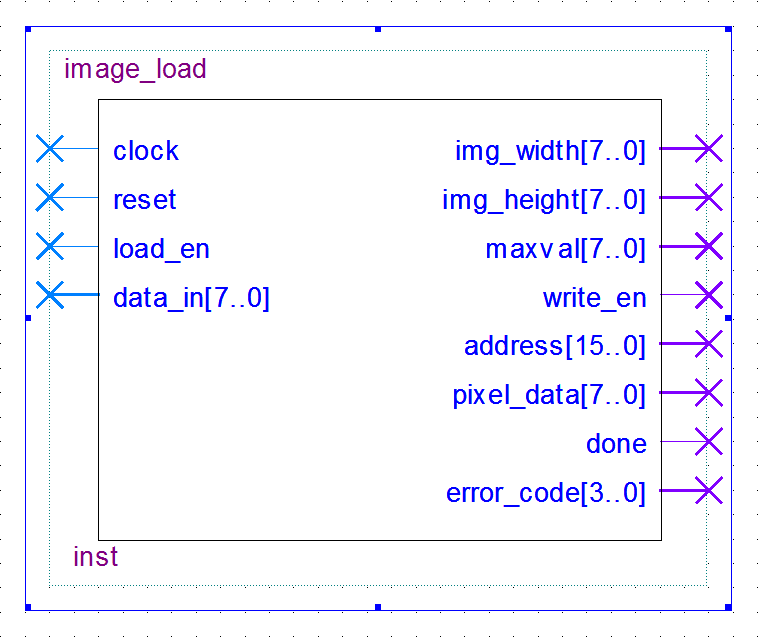
\includegraphics[width=0.5\linewidth]{image_load_entity.PNG}
    \caption{A module that loads PGM images from files into memory.}
    \label{fig:image_load}
\end{figure}

\begin{table}
    \centering
    \begin{tabular}[c]{ l | c | p{8cm} }
        \textbf{Error Name} & \textbf{Error Code} & \textbf{Description} \\
        \hline
        NONE & 0000 & No error has been encountered. \\
        INVALID\_FILETYPE & 0001 & The P2 file-type specifier was not found. \\
        WIDTH\_TOO\_LARGE & 0010 & The width exceeds 255. \\
        HEIGHT\_TOO\_LARGE & 0011 & The height exceeds 255. \\
        MAXVAL\_TOO\_LARGE & 0100 & The maxval exceeds 255. \\
        PIXEL\_TOO\_LARGE & 0101 & A pixel exceeds maxval. \\
        TOO\_MANY\_PIXELS & 0110 & The module has read more than width $\cdot$ height pixels. \\
        TOO\_FEW\_PIXELS & 0111 & The end of the file has been reached with less than width $\cdot$ height pixels read. \\
        INVALID\_TOKEN & 1000 & The module has encountered an unexpected character. \\
    \end{tabular}
    \caption{Possible IO errors encountered when parsing a PGM file.}
    \label{tab:io_error}
\end{table}

A pin-out of the image save module is shown in Figure \ref{fig:image_save}. The design also uses a datapath/controller system to output a PGM image to a file byte by byte. The img\_width, img\_height and maxval inputs are used to read in the image metadata, and the read\_en and address outputs are used to interface with an SRAM memory block and obtain the pixel\_data input. The module is enabled by the save\_en flag, and is reset with the asynchronous reset input. On each rising clock edge, the module can output an ASCII character on the data\_out line. It indicates that the character should be saved to a file through the write\_en flag. Finally, the done flag is used to indicate that the module has finished outputting all the data. Internally, the component stores the input data into a register. It then uses a binary to BCD conversion circuit and outputs each digit of the data on separate clock cycles after converting it to ASCII.

\begin{figure}
    \centering
    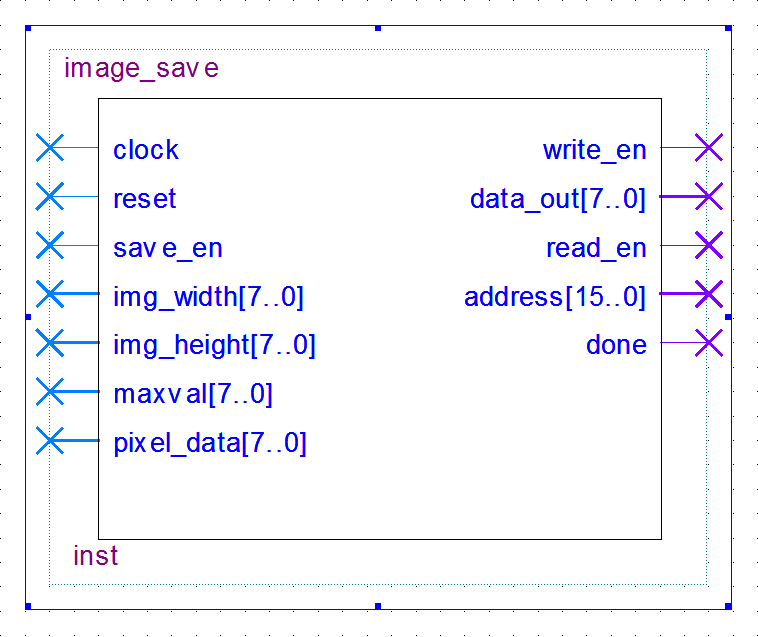
\includegraphics[width=0.5\linewidth]{image_save_entity.PNG}
    \caption{A module that saves PGM images from memory into files.}
    \label{fig:image_save}
\end{figure}

\subsection{Pixel Processor}

Next, the basic unit of pixel processing was designed. In addition to the operations specified, the absolute difference operation was added in order to better implement an edge detection algorithm. In addition, it was decided that the addition and subtraction operations should threshold the results at maxval and 0 respectively, as these behaviors make more sense in the context of pixel manipulation. This implementation also makes all data output by the processor valid. A description of the supported operations is given in Table \ref{tab:pixel_operations}. The pin-out diagram is shown in Figure \ref{fig:pixel_processor}. The data inputs are placed on the pixel\_data and pixel\_operand signals, the operation placed on the operation signal and the image maxval placed on the maxval signal. On each rising clock edge, data\_out is set to the result if enable is set. The data\_ready flag indicates that the data can be stored back in memory, and is included for potential pipelining of more complex operations in the future. The data\_valid flag indicates if the data is a valid pixel or if an overflow error has occurred. Currently, both of these flags are not used since the module operates in a single clock cycle and the data is always valid.

\begin{figure}
    \centering
    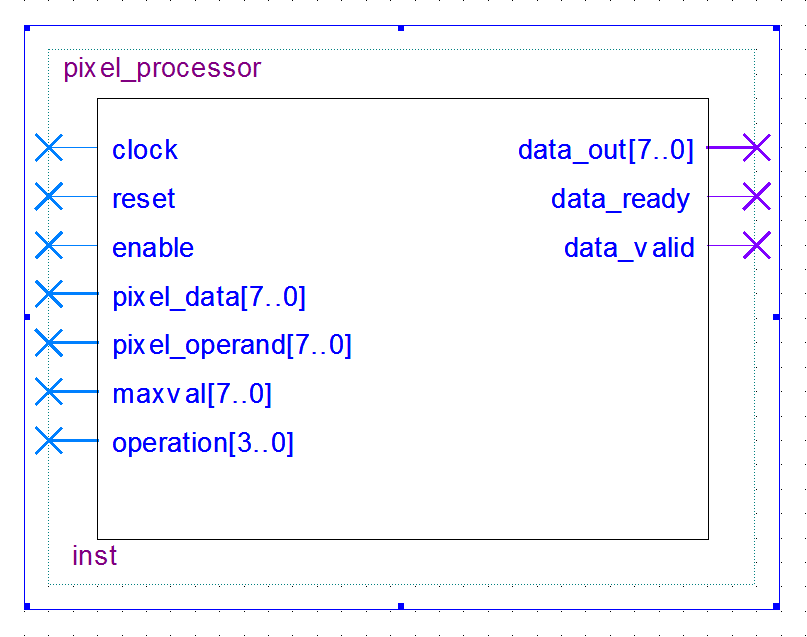
\includegraphics[width=0.5\linewidth]{pixel_processor_entity.PNG}
    \caption{A basic processing unit capable of performing pixel by pixel operations.}
    \label{fig:pixel_processor}
\end{figure}

\begin{table}
    \centering
    \begin{tabular}[c]{ l | c | p{10cm} }
        \textbf{Op Name} & \textbf{Op Code} & \textbf{Description} \\
        \hline
        SET & 0000 & Sets the output to the value of pixel\_operand. \\
        ADD & 0001 & Adds pixel\_data and pixel\_operand, capping the result at maxval. \\
        SUB & 0010 & Subtracts pixel\_operand from pixel\_data, capping the result at 0. \\
        AND & 0011 & Performs a bitwise AND on pixel\_data and pixel\_operand. \\
        OR & 0100 & Performs a bitwise OR on pixel\_data and pixel\_operand. \\
        XOR & 0101 & Performs a bitwise XOR on pixel\_data and pixel\_operand. \\
        INVERT & 0110 & Sets the output to maxval - pixel\_data. \\
        THRESH & 0111 & Sets the output to maxval if pixel\_data $>$ pixel\_operand, and to pixel\_data otherwise. \\
        ABSDIFF & 1000 & Outputs the absolute difference of pixel\_data and pixel\_operand. \\
    \end{tabular}
    \caption{Possible pixel operations performable by the pixel processor.}
    \label{tab:pixel_operations}
\end{table}

\subsection{Image Processor}

Finally, the image processor was designed using the modules defined previously. The pin-out diagram is shown in Figure \ref{fig:image_processor}. The processor was designed to be able to perform general purpose operations on images stored in 3 SRAM registers. The instruction to execute is specified by the reg\_in\_0, reg\_in\_1, reg\_out, global\_operand, address\_increment and operation signals. The types of operations are described in Table \ref{tab:image_operations}. The registers can be any of 00, 01 or 10, and the reg\_in\_1 input can take the special value 11 which indicated that the value of global\_operand should be used for all pixels in the register. The address\_increment input allows for horizontal left shifting of operation results, with the right-most columns being padded with the last value in each row. The module also includes the data\_in\_load and read\_en\_load inputs to provide an interface with the image load module, and the data\_out\_save and write\_en\_save outputs to provide an interface with the image save module. Finally, the done and error\_code signals specify the state of the processor, with the error codes being the same as those for the image load module.

\begin{figure}
    \centering
    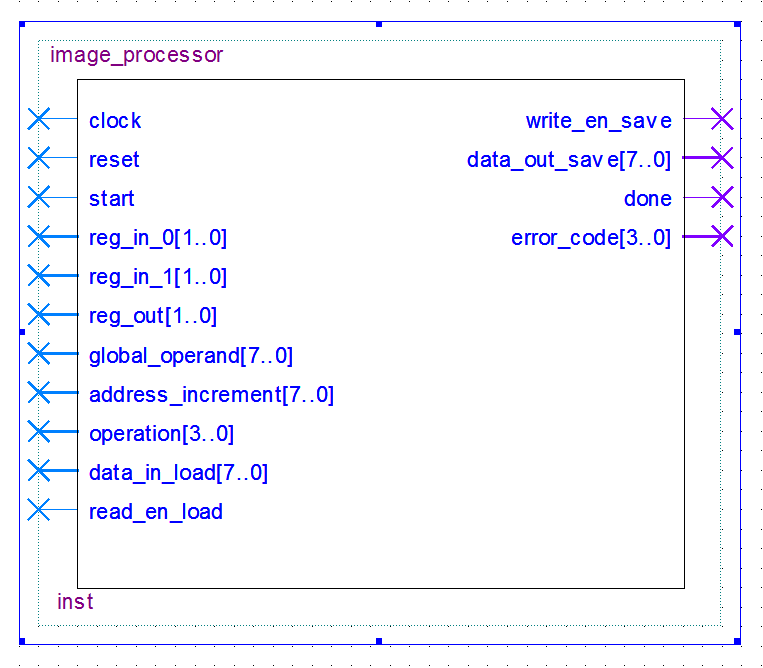
\includegraphics[width=0.5\linewidth]{image_processor_entity.PNG}
    \caption{A processing unit capable of performing pixel by pixel operations on images.}
    \label{fig:image_processor}
\end{figure}

\begin{table}
    \centering
    \begin{tabular}[c]{ l | c | p{10cm} }
        \textbf{Op Name} & \textbf{Op Code} & \textbf{Description} \\
        \hline
        SET & 0000 & reg\_out $\Leftarrow$ reg\_in\_1 \\
        ADD & 0001 & reg\_out $\Leftarrow$ reg\_in\_0 + reg\_in\_1, capped at maxval \\
        SUB & 0010 & reg\_out $\Leftarrow$ reg\_in\_0 - reg\_in\_1, capped at 0 \\
        AND & 0011 & reg\_out $\Leftarrow$ reg\_in\_0 AND reg\_in\_1 \\
        OR & 0100 & reg\_out $\Leftarrow$ reg\_in\_0 OR reg\_in\_1 \\
        XOR & 0101 & reg\_out $\Leftarrow$ reg\_in\_0 XOR reg\_in\_1 \\
        INVERT & 0110 & reg\_out $\Leftarrow$ maxval - reg\_in\_0 \\
        THRESH & 0111 & reg\_out $\Leftarrow$ reg\_in\_0 $>$ reg\_in\_1 ? maxval : reg\_in\_0 \\
        ABSDIFF & 1000 & reg\_out $\Leftarrow$ abs(reg\_in\_0 - reg\_in\_1) \\
        LOAD & 1001 & reg\_out $\Leftarrow$ file\_in \\
        SAVE & 1010 & file\_out $\Leftarrow$ reg\_in\_0 \\
    \end{tabular}
    \caption{Possible image operations performable by the image processor.}
    \label{tab:image_operations}
\end{table}

\subsection{Vertical Edge Detector}

The vertical edge detector was implemented as a test-bench that makes use of the image processor described above. It loads the main file to be processed into reg0 and the background into reg1, takes the difference and shifts it by 1 and stores the result in reg1, then performs an absolute difference between the two and thresholds the result with a threshold of 7. Then, it saves the result to a separate file. With this sequence of operations, no normalization is needed since the absolute difference operation cannot overflow. In addition, the rightmost column keeps its value when the image is shifted left, so the gradient will always be 0 on that column.

\section{Simulation Results}

% read/write image files...
% pixel operations
% SUB, XOR, THRES images
% EDGE DETECTOR

\section{Synthesis Results}

FPGA: Cyclone V 5CSEMA5F31C6N

\end{document}
